\subsection{Interpolation}
Let $p$ refer to an arbitrary patient whose pain score records started less than two hours post-operation. Since pain scores were recorded at inconsistent intervals, it is necessary to standardize them to consistent intervals. Ten minutes was chosen as the standard interval between scores, and recorded scores were linearly interpolated  and estimated for these periods. Figure \ref{fig:interpolation} illustrates the transformation from sample recorded scores, \eqref{eqn:recorded_scores}, to interpolated scores, \eqref{eqn:interpolated_scores} (rounded to the hundredths place for display purposes).

\begin{equation}\label{eqn:recorded_scores}
    recorded=(3\ minutes: 4, 24\ minutes: 8, 45\ minutes: 4, 100\ minutes: 2)
\end{equation}

\begin{equation}\label{eqn:interpolated_scores}
\begin{split}
    interpolated=(&3\ minutes:4.0, 13\ minutes:5.9, 23\ minutes:7.8,\\
                  &33\ minutes:6.3, 43\ minutes:4.4, 53\ minutes:3.7,\\
                  &63\ minutes:3.3, 73\ minutes:3.0, 83\ minutes:2.6,\\
                  &93\ minutes:2.0)
\end{split}
\end{equation}

\begin{figure}[h]
  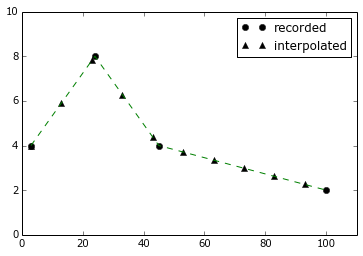
\includegraphics[scale=0.4]{./Figures/interpolation.png}\\
  \caption{Illustration of interpolation procedure. Recorded pain scores are connected via a linear function of time from which interpolated scores are predicted at consistent, ten-minute intervals.}\label{fig:interpolation}
\end{figure}

Denote patient $p$'s time series of 10-minute interpolated pain scores as $\tilde{S}=(s_1,...,s_d)$, where the $t$'th item is the estimated pain score $10(t-1)$ minutes past the first recorded score, and $d=floor\left(\frac{max(recording time)}{10}\right)$. So $s_1$ is the first pain score recorded for that patient with subsequent elements estimated from linear interpolation, and $d$ is the index of the last available data point estimated from interpolation without forecasting past the last recorded pain score. For the example interpolated values in \eqref{eqn:interpolated_scores}, $\tilde{S}=(4.0, 5.9, 7.8, 6.3, 4.4, 3.7, 3.3, 3.0, 2.6, 2.3)$. 